\chapter{Generic EPS Component Models}
\label{appendix:eps-component-models}

The CSRM logical components represent generic component types that mission teams refine into physical designs \citep{kaslow2019csrm}.
For these EPS categories, this appendix uses ``function'' and ``logical component'' interchangeably.
Interfaces are modeled as component properties that depend on the properties of other EPS components.
The figures present the complete declared component properties, modes, states and requirement assignment for the third objective.
All numerical examples are illustrative allocations.

\begin{figure}[htbp]
\centering
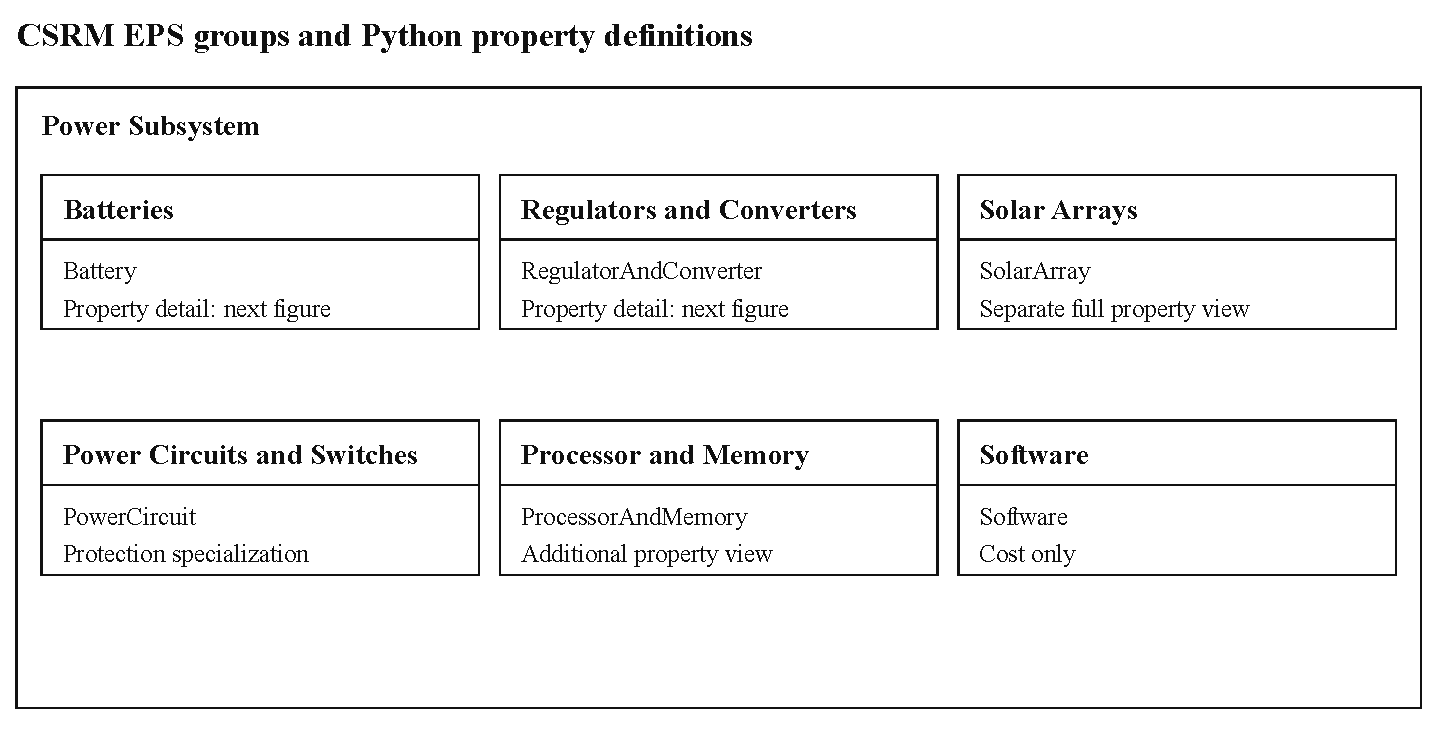
\includegraphics[width=\linewidth]{fig/model-appendices/eps-property-structure.pdf}
\caption[CSRM EPS categories and their Python classes.]{A property-oriented variant of Figure~\ref{fig:csrm-eps-components}. The six group names follow the CSRM reference model \citep{incose2025csrmmodel}. The numerical EPS model defines four default component classes and a Protection specialization. Processor and Memory, and Software, remain reference categories with no dedicated class or additional declared properties. Figures~\ref{fig:eps-component-properties}--\ref{fig:solar-array-properties} list the complete property definitions of the numerical classes.}
\label{fig:eps-property-structure}
\end{figure}
\clearpage

\begin{figure}[p]
\centering
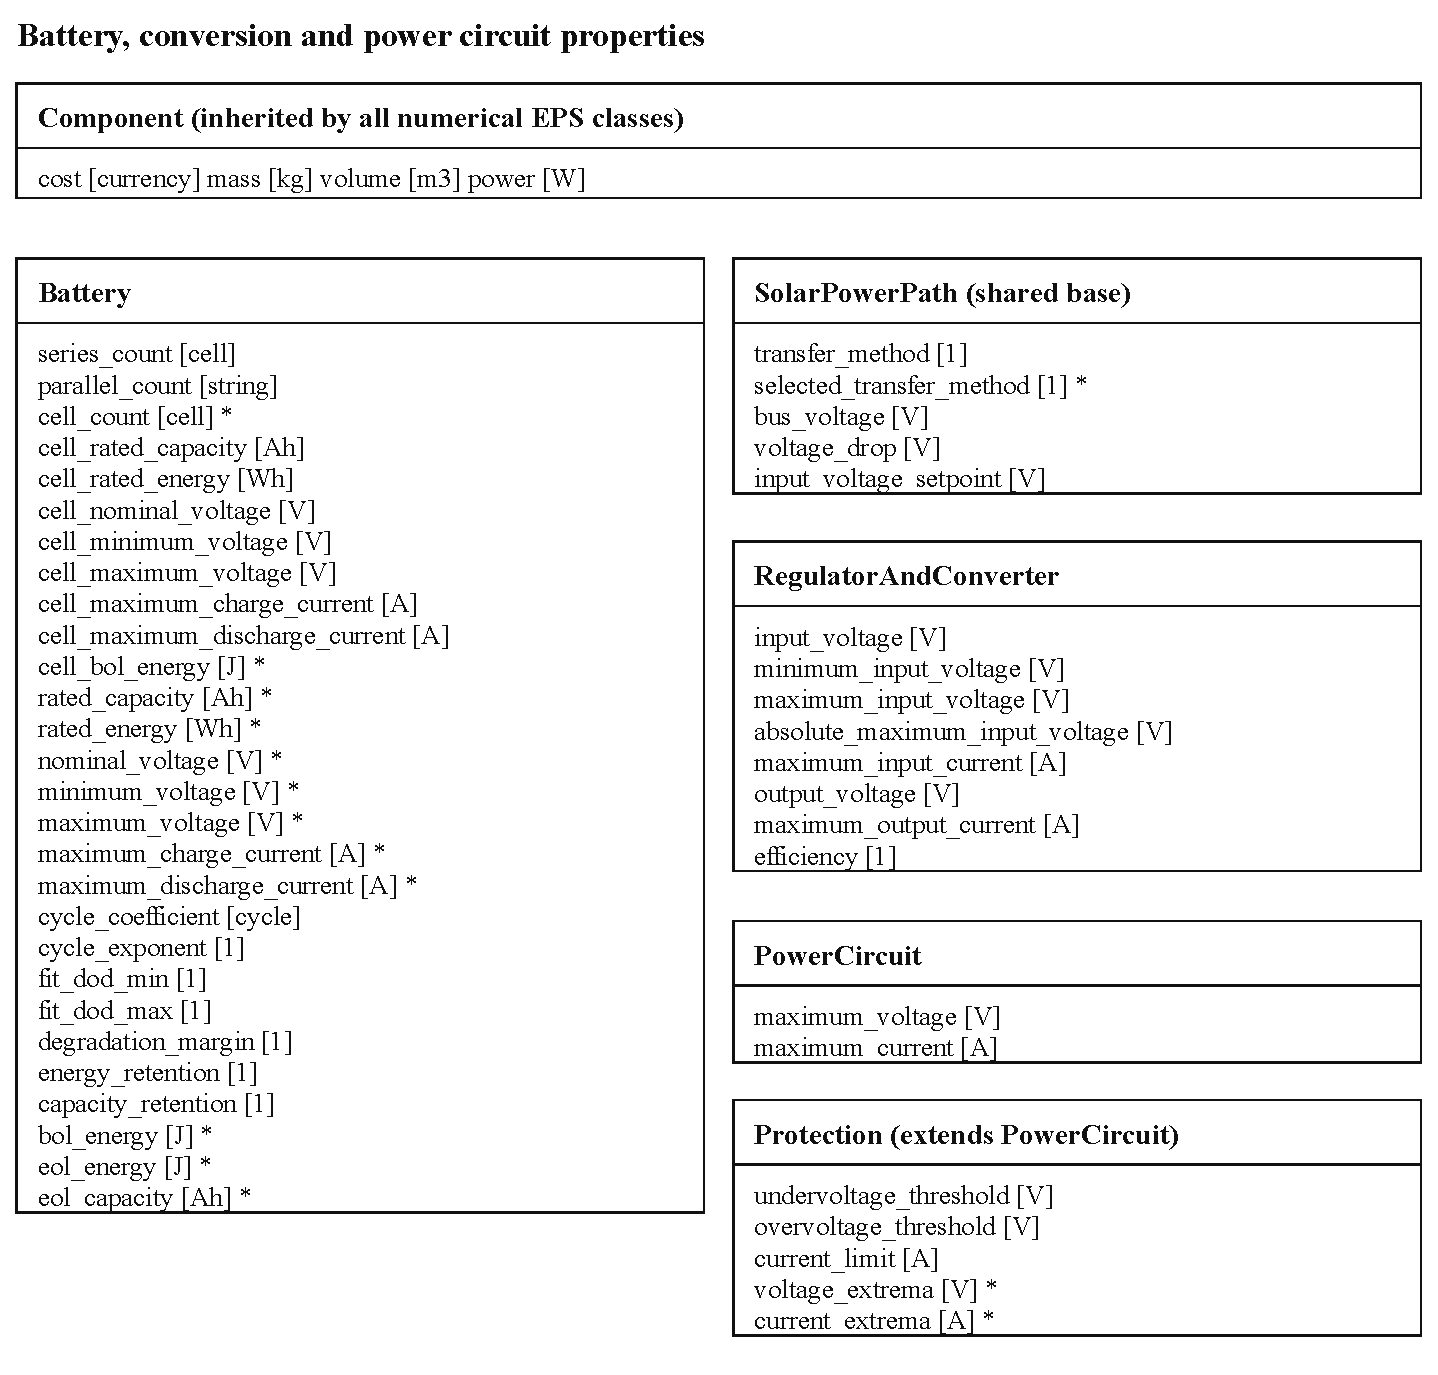
\includegraphics[width=\linewidth]{fig/model-appendices/eps-component-properties.pdf}
\caption[Battery, conversion and power circuit properties.]{Complete declared properties for Battery, RegulatorAndConverter, PowerCircuit and Protection. All inherit the four Component properties. RegulatorAndConverter and PowerCircuit also inherit SolarPowerPath properties, and Protection inherits PowerCircuit. Brackets retain the model's unit annotations, with 1 denoting a dimensionless value. An asterisk marks a supplied default expression. Other properties start unset. Units are annotations and receive no automatic conversion or dimensional checking.}
\label{fig:eps-component-properties}
\end{figure}
\clearpage

\begin{figure}[p]
\centering
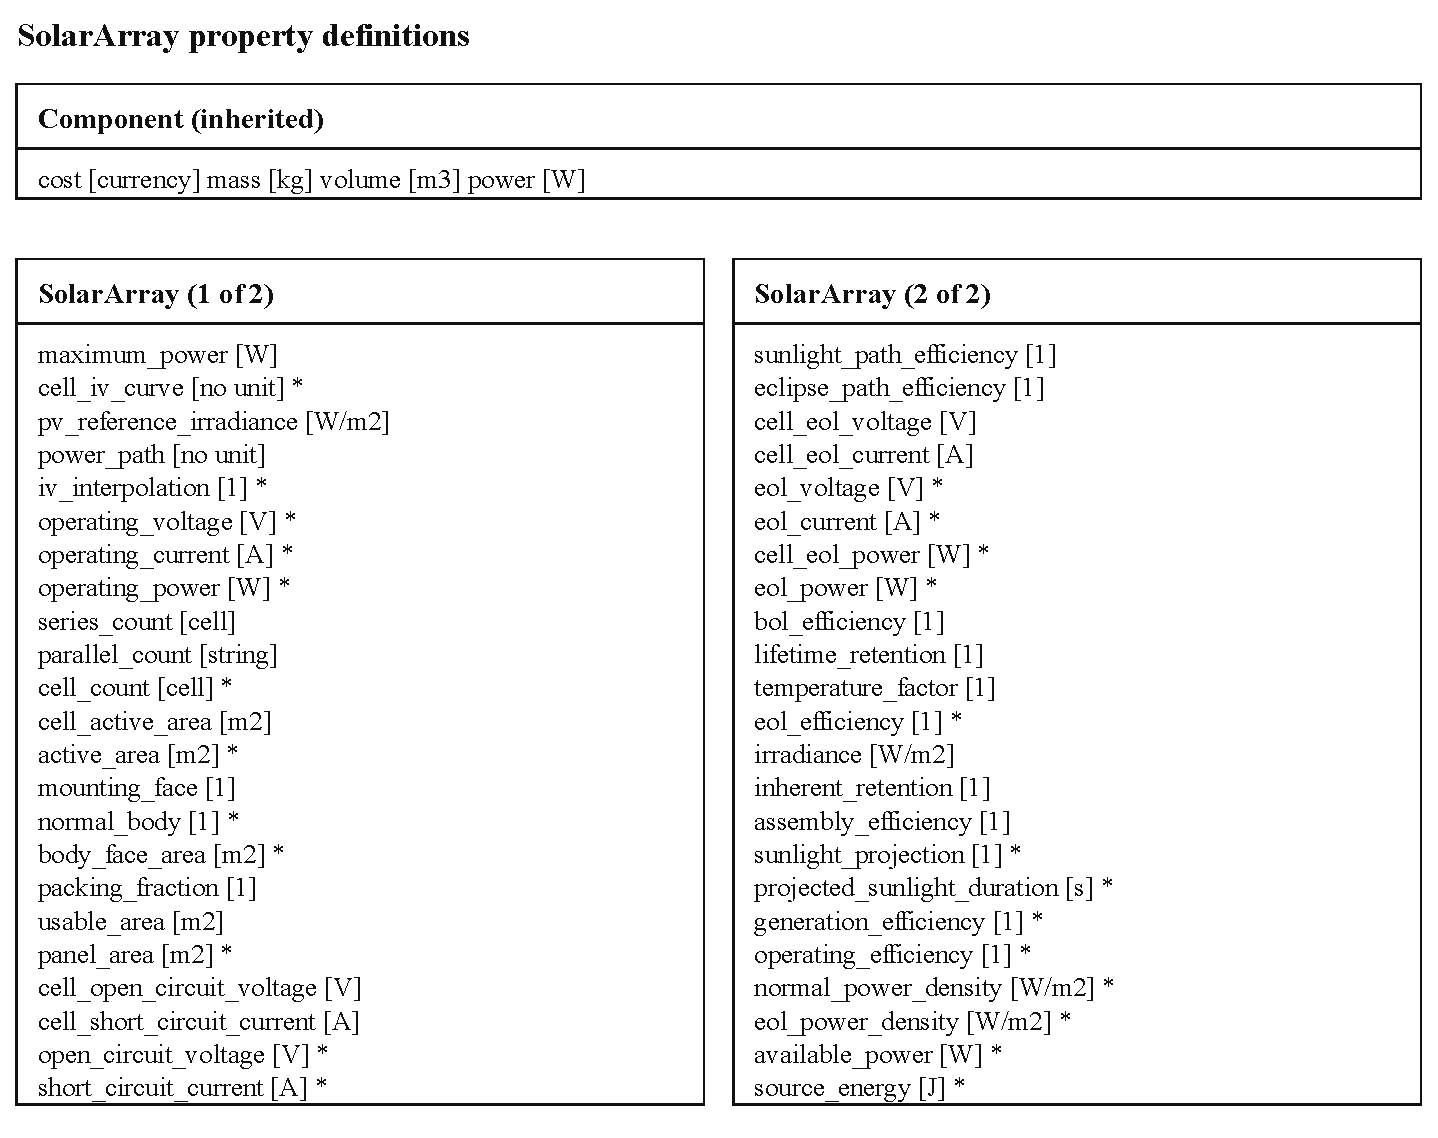
\includegraphics[width=\linewidth]{fig/model-appendices/solar-array-properties.pdf}
\caption[Complete solar array properties.]{The complete SolarArray property list, split across two columns for readability. The Component properties are inherited. Brackets and asterisks follow Figure~\ref{fig:eps-component-properties}. ``No unit'' denotes a property without a unit annotation, such as the selected power path reference or a collection of photovoltaic points. The default expressions retain explicit dependencies on orbit, attitude, installation geometry and the selected electrical path.}
\label{fig:solar-array-properties}
\end{figure}
\clearpage

\begin{figure}[p]
\centering
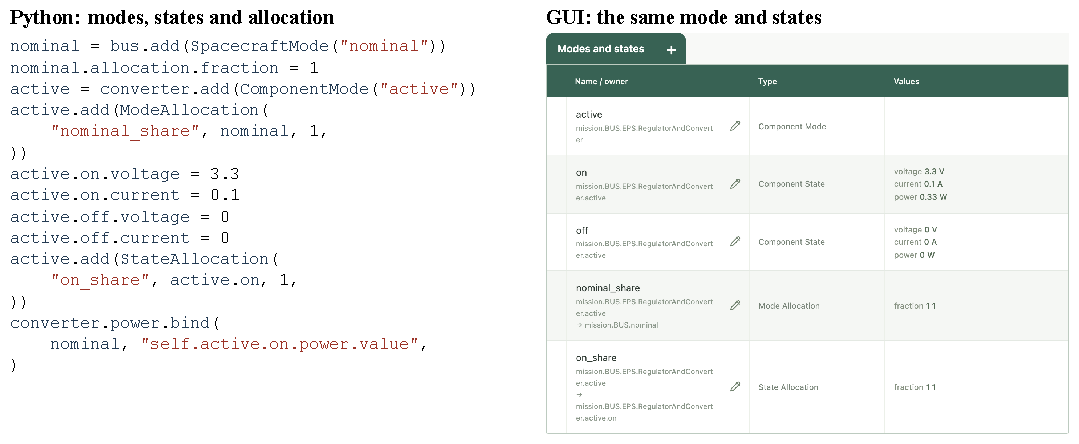
\includegraphics[width=\linewidth]{fig/model-appendices/modes-and-states.pdf}
\caption[Component modes and states in Python and the GUI.]{The Python definition is on the left and the live GUI view is on the right. Adding a ComponentMode creates its on and off ComponentState objects. Each state has voltage, current and a power expression equal to their product. The on state evaluates to 0.33~W and the off state to 0~W. ModeAllocation links the component mode to the spacecraft mode, and StateAllocation records an explicit state fraction. The power binding selects the on state for nominal evaluation. Allocations impose no automatic averaging, normalization or chronological simulation.}
\label{fig:eps-modes-states}
\end{figure}

\begin{figure}[p]
\centering
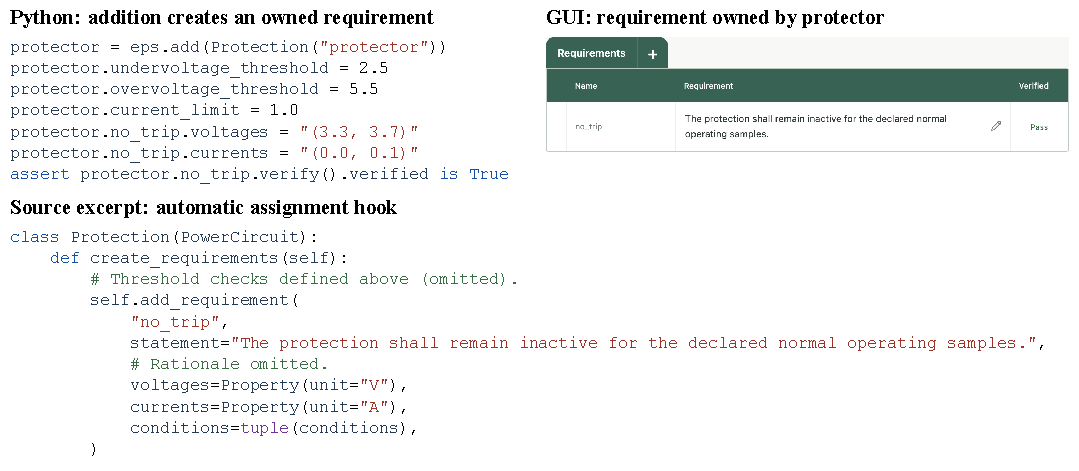
\includegraphics[width=\linewidth]{fig/model-appendices/requirement-assignment.pdf}
\caption[Automatic requirement assignment to an EPS component.]{Adding the Protection component invokes its create\_requirements() method and assigns its owned no\_trip requirement. The source excerpt retains the assignment call and omits the construction of its threshold checks and rationale. The live GUI on the right shows the resulting requirement passing for the supplied normal operating samples. EPS requirements use the same ownership mechanism and are listed in Appendix~\ref{appendix:automatic-eps-requirements}. Authored requirement assignment is illustrated in Figure~\ref{fig:mission-requirement-operations}.}
\label{fig:eps-requirement-assignment}
\end{figure}
\clearpage

\begin{figure}[p]
\centering
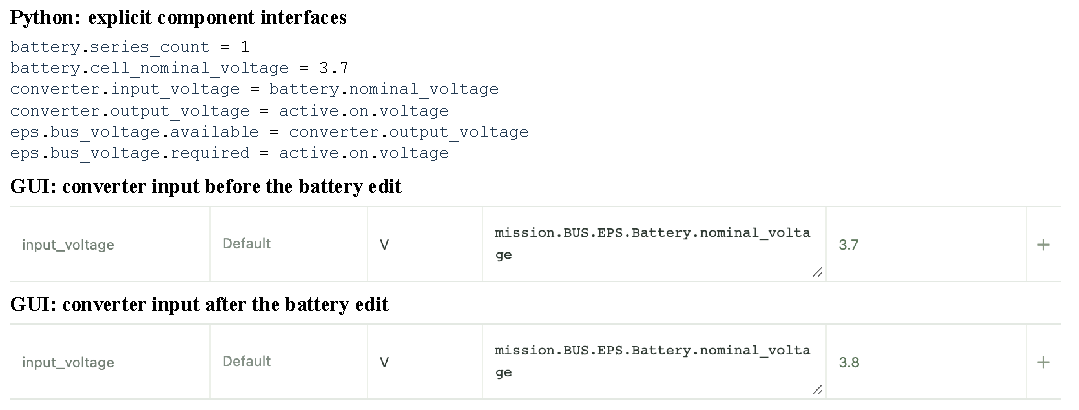
\includegraphics[width=\linewidth]{fig/model-appendices/property-interfaces.pdf}
\caption[Interfaces expressed as dependent component properties.]{The converter input voltage references the battery nominal voltage, and the converter output and EPS load requirement reference the selected load state. The two live GUI rows show the converter's unchanged input expression before and after changing the battery cell nominal voltage from 3.7~V to 3.8~V. Its evaluated input voltage changes through the stored dependency. These explicit links describe the chosen electrical interface and establish no automatic wiring or circuit synthesis.}
\label{fig:eps-property-interfaces}
\end{figure}
\clearpage
